\documentclass{uai2026} % anonymous submission (class strips author block)
% \documentclass[accepted]{uai2026} % preview non-anonymous version

\usepackage[american]{babel}
\usepackage{natbib}
    \bibliographystyle{plainnat}
    \renewcommand{\bibsection}{\subsubsection*{References}}
\usepackage{mathtools}
\usepackage{amssymb}
\usepackage{booktabs}
\usepackage{tikz}

% Convenience macros
\newcommand{\ROAS}{\mathrm{ROAS}}
\newcommand{\bbE}{\mathbb{E}}
\newcommand{\dosym}{\mathrm{do}}

\title{Experiment-Calibrated Media Mix Models: Bayesian Fusion of Interventional and Observational Evidence for Marketing Decision-Making}

\author[1]{\href{mailto:juan.orduz@pymc-labs.com?Subject=Your UAI 2026 paper}{Juan~Orduz}{}}
\affil[1]{%
    PyMC Labs\\
    Principal Data Scientist
}

\begin{document}
\maketitle

\begin{abstract}
  Marketing-mix models (MMMs) allocate large advertising budgets across channels yet are fit on observational time series in which spend is correlated with unobserved drivers of revenue and with other channels through shared launch windows.
  We frame budget allocation as off-policy evaluation under partial identifiability and show how interventional evidence from geo-lift and conversion-lift experiments can be fused with the observational MMM as an additional saturation-curve likelihood term, rather than as a prior on uninterpretable regression coefficients.
  In a controlled simulation the naive observational model roughly doubles the implied effect of the confounded channel; calibration via lift-test likelihood recovers the channel-level return-on-ad-spend in tight credible intervals around ground truth, and we evaluate it in policy space against an oracle allocator with a sensitivity analysis over the experimental prior.
  The recipe is a deployable instance of causal data fusion for decision making under unobserved confounding, open-sourced in PyMC-Marketing.
\end{abstract}

\section{Introduction}\label{sec:intro}

A retailer choosing how to split an annual advertising budget across paid search, paid social, video, display, and other channels is solving a sequential decision problem under partial identifiability.
The value of any candidate allocation depends on causal effects (the incremental revenue produced by an additional dollar of spend on each channel), which observational time series alone cannot identify whenever spend is correlated with unobserved drivers of the outcome.
This is the default rather than the exception: marketers raise budgets in periods of strong demand, react to competitors, and follow seasonal or macroeconomic signals that the model never sees.
The identification problem is not only about unobserved confounders: in strongly seasonal businesses (food delivery, retail flash sales, travel), paid search, paid social, video, and display are often activated together around the same demand peaks, and this co-activation alone is enough to leave channel-level effects weakly identified before any latent driver is introduced.
We frame the problem as off-policy evaluation in a contextual setting where the logging policy is the marketer's historical behavior, confounded by these unobserved factors \citep{dudik2014ope}.

Standard media-mix models (MMMs) are Bayesian regressions that combine adstock and saturation transformations of channel spend with controls for trend and seasonality \citep{jin2017bayesian,salvatier2016pymc,pymcmarketing2024}.
They produce posterior intervals on regression coefficients and on derived quantities such as channel return-on-ad-spend (ROAS).
When relevant confounders are unobserved, however, the resulting estimates are biased in a direction that the model itself cannot diagnose, and the bias propagates directly into the chosen allocation.
In the controlled simulation of Section~\ref{sec:experiments}, a naive observational MMM roughly doubles the channel-level effect of a confounded channel, which is enough to reverse the ranking of channels by ROAS.
Goodness of fit on held-out windows is uninformative about this failure \citep{vincent2026goodnessfit,orduz2026nor2}.

Geo-lift experiments, conversion-lift studies, and switchback designs provide local interventional evidence on a subset of channels at a subset of time points.
We treat the resulting lift estimates as observations of the saturation curve at known spend pairs and add them to the MMM as a likelihood term, fusing observational and interventional evidence in a single posterior \citep{bareinboim2016causal,colnet2024causal}.
Our contributions are:
(i)~a structural causal formulation of the standard MMM that makes the identification gap explicit;
(ii)~a calibration likelihood on incremental ROAS that places experimental evidence on the policy-relevant causal estimand rather than on a model-internal nuisance coefficient;
(iii)~an evaluation in policy space, instantiated through a constrained-optimization pipeline that admits both expected-revenue and risk-aware Bayesian objectives, and reporting the revenue gap that calibration closes between a naive policy and the oracle policy that knows the confounder; and
(iv)~a sensitivity analysis quantifying how decision loss degrades when the experimental evidence is biased or stale.
A reference implementation ships with PyMC-Marketing.

\section{Problem Setup and Causal Framing}\label{sec:setup}

We index time by $t = 1,\dots,T$.
Let $X_t \in \mathbb{R}_{\ge 0}^K$ be the spend vector across $K$ channels, $W_t$ a vector of observed controls (seasonality, calendar effects, promotions), $Z_t$ a vector of unobserved confounders, and $Y_t$ the outcome (revenue or conversions).
The structural causal model is shown in Figure~\ref{fig:dag}.

\begin{figure}[!tb]
  \centering
  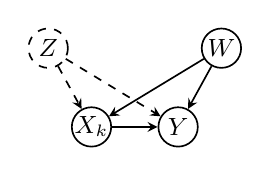
\begin{tikzpicture}[
    every node/.style={circle, draw, minimum size=5mm, inner sep=0pt, font=\small},
    >=stealth, semithick
  ]
    \node[dashed] (Z) at (0, 1.0) {$Z$};
    \node (W) at (2.2, 1.0) {$W$};
    \node (X) at (0.55, 0) {$X_k$};
    \node (Y) at (1.65, 0) {$Y$};
    \draw[->, dashed] (Z) -- (X);
    \draw[->, dashed] (Z) -- (Y);
    \draw[->] (W) -- (X);
    \draw[->] (W) -- (Y);
    \draw[->] (X) -- (Y);
  \end{tikzpicture}
  \caption{SCM for the MMM. Dashed arrows from unobserved $Z$ open the backdoor $X_k \leftarrow Z \to Y$ that conditioning on the observed $W$ cannot close.}\label{fig:dag}
\end{figure}
Following the standard MMM specification \citep{jin2017bayesian}, the outcome equation is
\begin{multline}\label{eq:scm}
    Y_t = f_\text{trend}(t) + g(W_t) + h(Z_t) + \varepsilon_t \\
    + \sum_{k=1}^{K} \beta_k\, S_{\lambda_k}\!\bigl(A_{\alpha_k}(X_{k,1:t})\bigr),
\end{multline}
where $A_{\alpha_k}$ is an adstock transform with decay $\alpha_k$ (here geometric, but any of the standard families applies), $S_{\lambda_k}$ a saturation transform with shape $\lambda_k$ (logistic, Hill, Michaelis-Menten, \dots), and $\varepsilon_t$ Gaussian noise.
Adstock and saturation are part of the structural equation, not preprocessing.

The causal contrast of interest is the channel-level intervention effect $\bbE[Y_t \mid \dosym(X_{k,t} = x)] - \bbE[Y_t \mid \dosym(X_{k,t} = 0)]$.
Conditioning on $W_t$ alone does not identify it whenever any component of $Z_t$ remains unobserved: the backdoor path $X_{k,t} \leftarrow Z_t \to Y_t$ stays open, and the regression coefficient $\beta_k$ in (\ref{eq:scm}) absorbs both the causal effect and the confounding contribution of $Z_t$.
This is the central practical difficulty of MMM: relevant confounders, such as latent demand, supply shocks, competitor behaviour, and price changes, are pervasive and rarely observed.
A second, mechanical source of the problem is multicollinearity in $X_t$ itself: because campaigns are typically launched on the same calendar windows, the spend columns share common variation, enlarging the posterior ridge in coefficient space and amplifying any bias that the unobserved $Z_t$ already introduces.

The decision-maker cares not about $\beta_k$ but about the channel-level ROAS evaluated at a candidate spend trajectory $x_{k,1:T}$,
\begin{equation}\label{eq:roas}
    \ROAS_k(x_{k,1:T}) = \frac{\sum_t \bbE\!\bigl[Y_t(x_{k,1:t}) - Y_t(0)\bigr]}{\sum_t x_{k,t}},
\end{equation}
which is the same quantity that a geo-lift or conversion-lift experiment estimates.
Given a total budget $B$, an allocator chooses $\hat\pi \in \mathbb{R}_{\ge 0}^K$ with $\sum_k \hat\pi_k = B$ to maximize expected revenue under the posterior over $(\alpha_k, \lambda_k, \ROAS_k)$.
Writing $V(\pi) = \bbE_{p^\star}\!\bigl[Y \mid \dosym(X = \pi)\bigr]$ for the expected outcome under the true data-generating process $p^\star$ when the spend policy is $\pi$, we measure decision loss as the revenue gap to the oracle allocator,
\begin{equation}\label{eq:loss}
    \Delta R(\hat\pi) = V(\pi^\star) - V(\hat\pi).
\end{equation}
This is the metric we report (\ref{eq:loss}): not RMSE on $\beta_k$, not coverage of credible intervals, but expected money left on the table.

\section{ROAS-Parameterized Framework}\label{sec:method}

The natural Bayesian response to confounding is to use informative priors on $\beta_k$, but $\beta_k$ is a coefficient on a transformed and rescaled spend channel whose scale depends on the adstock decay $\alpha_k$, the saturation shape $\lambda_k$, and any standardization of the data; experiments produce evidence on incremental revenue per unit spend, with no direct mapping to $\beta_k$ without first knowing the nuisance parameters, so prior elicitation in coefficient space is not even well-defined in practice.
Following \citet{wurm2024mmmcalibration}, we reparameterize the model so that channel ROAS is a primitive parameter and $\beta_k$ is derived deterministically.
For each posterior draw of $(\alpha_k, \lambda_k, \ROAS_k)$ and given the observed spend trajectory $X_{k,1:T}$, we compute
\begin{equation}\label{eq:roas-beta}
    \beta_k \;=\; \ROAS_k \cdot \frac{\sum_{t=1}^T X_{k,t}}{\sum_{t=1}^T S_{\lambda_k}\!\bigl(A_{\alpha_k}(X_{k,1:t})\bigr)},
\end{equation}
so that the posterior over $\ROAS_k$ is the object of inference and $\beta_k$ inherits its scale from the saturation transform.
This is a domain-specific instance of decoupling the causal target from the nuisance parameters that link it to the observed data \citep{evans2024frugal,orduz2024frugal}.

Prior elicitation now operates on a quantity that practitioners reason about in orders of magnitude.
When several lift experiments are available on the same channel, \citet{wurm2024mmmcalibration} recommend a weighted sum of the per-experiment ROAS priors with weights proportional to experimental spend; this discards the spend-level information each experiment carried about the saturation curve, which the per-experiment likelihood of Section~\ref{sec:liftlik} retains by anchoring each test at the spend pair where it was measured.
The reparameterization alone is not yet calibration: the posterior on $\ROAS_k$ still inherits the bias of the observational likelihood whenever $Z_t$ is unobserved, which is what the interventional evidence corrects.

\section{Calibration via Lift-Test Likelihood}\label{sec:liftlik}

A geo-lift or conversion-lift experiment on channel $k$ produces a tuple $(x, \Delta x, \Delta y, \tau)$: the baseline spend $x$ on the same scale as the MMM's input, the spend change $\Delta x$ delivered by the experiment, the estimated outcome lift $\Delta y$, and the experiment's reported uncertainty $\tau$ on $\Delta y$ (a scale parameter, distinct from the observational-noise scale of $\varepsilon_t$).
The lift is a finite-difference observation of the saturation curve at two known spend levels.
We add it to the model as a positive-support likelihood on the magnitude of the finite-difference lift,
\begin{multline}\label{eq:lift-lik}
    |\Delta y| \;\sim\; \mathrm{Gamma}\bigl(\mu_k,\, \tau\bigr),\\
    \mu_k = \bigl|S_{\lambda_k}\!\bigl(A_{\alpha_k}(x + \Delta x)\bigr) - S_{\lambda_k}\!\bigl(A_{\alpha_k}(x)\bigr)\bigr|,
\end{multline}
using the same adstock and saturation transforms that already appear in (\ref{eq:scm}) and PyMC's $(\mu,\sigma)$ parametrization of the Gamma distribution (with $\sigma \equiv \tau$).
The absolute value lets the likelihood accommodate either sign of measured lift on a single positive-support distribution and matches the default implementation in PyMC-Marketing \citep{pymcmarketing_lift_test_source}; a Normal alternative is exposed by the same API for use cases where signed lifts and symmetric uncertainty are preferred.
Equation (\ref{eq:lift-lik}) is independent of the specific adstock and saturation families chosen in (\ref{eq:scm}): it only requires that $S_{\lambda_k}(A_{\alpha_k}(\cdot))$ can be evaluated at the two spend levels of the experiment, so the recipe transfers without modification to any MMM whose adstock/saturation transforms are differentiable.
Multiple lift tests on the same or different channels enter as independent likelihood terms whose product multiplies the observational likelihood.
The full posterior fuses the two sources of evidence and produces a single coherent uncertainty over $(\alpha_k, \lambda_k, \ROAS_k)$ for every channel.

The likelihood form (\ref{eq:lift-lik}) places experimental evidence on the saturation curve, which the regression component cannot identify without it.
A single lift test still leaves a one-dimensional ridge in the $(\lambda_k, \beta_k)$ plane: the same $\Delta y$ is consistent with a low-saturation, high-coefficient curve and a high-saturation, low-coefficient curve, an identifiability issue documented by \citet{vincent2026liftasymptote}.
Two or more lift tests at different spend levels resolve the ridge.
In practice, even a single test moves the posterior decisively when combined with the observational data: it pins down the curve at one point and the regression component constrains the rest.

The strength of the calibration is governed by $\tau$.
A tight $\tau$ places strong weight on the experiment and shrinks the posterior toward the experimental measurement; a loose $\tau$ recovers the uncalibrated observational fit.
This is the Bayesian analogue of the power-prior dial \citep{ibrahim2000power}: $\tau$ interpolates between observational-only and experiment-only inference and admits a transparent practitioner interpretation.
Lift tests can also be aggregated hierarchically across geographies or campaigns, with channel-level $\ROAS_k$ as a partial-pooling target across studies, in the spirit of multiple randomization designs \citep{masoero2025multiple}.
The implementation in PyMC-Marketing exposes the calibration through a single \texttt{add\_lift\_test\_measurements} call \citep{pymcmarketing2024}, taking a dataframe with columns \texttt{(channel, x, delta\_x, delta\_y, sigma)}.

\section{Experiments}\label{sec:experiments}

\subsection{Synthetic Environment}\label{sec:synth}

We simulate $T=131$ weeks of data with $K=2$ channels.
Adstock is geometric with maximum lag $4$ and decays $(\alpha_1, \alpha_2) = (0.3, 0.5)$; saturation is logistic with shapes $(\lambda_1, \lambda_2) = (1.0, 2.5)$; coefficients are $(\beta_1, \beta_2) = (2.0, 1.5)$.
The unobserved confounder is $Z_t \sim \mathrm{Gamma}(1, 2/3)$ with effect $\beta_Z = 0.3$ and edges $Z_t \to X_{1,t}$ (channel 1 is confounded; channel 2 is not) and $Z_t \to Y_t$.
Trend is a cubic-root function of time, and seasonality is a Fourier basis of order one with annual period.
The implied ground-truth ROAS values, computed from the structural equation, are $\ROAS_1 \approx 93.4$ and $\ROAS_2 \approx 171.4$ on the original revenue scale.
We compare four model variants: an oracle model (M1) that observes $Z_t$ and establishes the achievable ceiling; a naive model (M2) that omits $Z_t$ and uses uninformative priors on $(\alpha_k, \lambda_k, \beta_k)$; a reparameterized model (M3) that omits $Z_t$ and parameterizes $\ROAS_k$ directly, with a LogNormal prior on $\ROAS_k$ built from aggregated experimental estimates following Wurm's weighted-sum recipe (this is the setup of the public PyMC-Marketing notebook \citealp{pymcmarketing_mmm_roas_parametrization}); and a calibrated model (M4) that omits $Z_t$, uses the same ROAS reparameterization, and additionally adds a per-experiment saturation-likelihood term (\ref{eq:lift-lik}) on each channel using lift estimates centered at the ground-truth ROAS values with $\tau = 30$ on the original scale (the setup of \citealp{pymcmarketing_mmm_roas}).
All models are fit in PyMC with NUTS via the \texttt{numpyro} backend.

\subsection{Estimation Results}\label{sec:estimation}

The naive model M2 inflates the channel-1 coefficient to $\hat\beta_1^{M2} = 1.485\,[0.915, 2.099]$, roughly double the oracle value $\hat\beta_1^{M1} = 0.709\,[0.262, 1.288]$, and absorbs the confounding contribution into the channel; translated through (\ref{eq:roas-beta}) onto the policy-relevant scale, this corresponds to a posterior $\widehat{\ROAS}_1^{M2}$ approximately twice the ground-truth $93.4$, the same factor-of-two bias visible in coefficient space.
On the unconfounded channel 2, the bias is small.
Under M3, the aggregated-experiment prior pulls the $\ROAS_k$ posteriors onto the right scale: the channel-1 posterior is centered near $95$ against ground truth $93.4$ and the channel-2 posterior near $170$ against ground truth $171.4$ \citep{pymcmarketing_mmm_roas_parametrization}.
Under M4, the per-experiment saturation likelihood tightens these posteriors further and concentrates them on ground truth, with credible intervals that contract progressively as more lift tests are incorporated \citep{pymcmarketing_mmm_roas}.
In this simulation M4 yields more accurate posteriors than M3, and both are directionally far closer to ground truth than M2, reversing the channel ranking that the naive fit would otherwise induce.

% TODO: include figures/fig3_posteriors.pdf once exported from the notebook
% \begin{figure}[!htb]
%   \centering
%   \includegraphics[width=\linewidth]{figures/fig3_posteriors}
%   \caption{Channel-level ROAS posteriors under M1 (oracle), M2 (naive), M3 (ROAS-reparameterized), and M4 (calibrated). Ground truth marked.}\label{fig:posteriors}
% \end{figure}

\subsection{Decision-Loss Evaluation}\label{sec:decision}

We compare four policies under a fixed total budget $B$: the oracle policy $\pi^\star$ under M1, the naive $\hat\pi^{M2}$, the reparameterized $\hat\pi^{M3}$, and the calibrated $\hat\pi^{M4}$.
Each policy solves a constrained nonlinear program (SLSQP) maximizing posterior expected revenue subject to $\sum_k \pi_k = B$ and per-channel bounds; the objective is evaluated by pushing $\pi$ through the posterior predictive of $S_{\lambda_k}(A_{\alpha_k}(\cdot))$, following the reference pipeline in PyMC-Marketing \citep{pymcmarketing_budget_allocation}.
The optimizer's only structural inputs are the saturation parameters $(\alpha_k, \lambda_k)$ and the ROAS posterior, so the calibration recipe of Section~\ref{sec:liftlik} is what unlocks the optimization rather than a downstream concern: a biased posterior on these objects produces a biased argmax no matter how well-tuned the solver.
The naive policy over-allocates to the confounded channel; both M3 and M4 reverse this and reproduce the oracle's ranking across a sweep of total budgets, with $\hat\pi^{M4}$ tracking the oracle most closely and closing a substantially larger fraction of $V(\pi^\star) - V(\hat\pi^{M2})$ than M3, the residual gap reflecting weak identification of the saturation shape.
% TODO: include figures/fig4_decision_loss.pdf
The same objective extends to a risk-aware Bayesian one trading mean response against tail risk in the posterior predictive (Value-at-Risk, or a mean-tightness criterion penalizing posterior dispersion); tighter, unbiased posteriors on the saturation curves translate directly into better risk-adjusted allocations, not only better expected-value ones \citep{pymcmarketing_allocation_assessment}.

\subsection{Sensitivity to Prior Misspecification}\label{sec:sensitivity}

Lift tests are themselves biased by spillover, market heterogeneity, and staleness, so we probe robustness by sweeping the experimental prior mean across $\{0.5, 0.75, 1.0, 1.25, 1.5\}\times \ROAS_k^\text{true}$ and the scale $\tau$ over a range, measuring decision loss (\ref{eq:loss}) for each combination.
% TODO: insert sensitivity heatmap (figures/fig5_sensitivity.pdf) once available.
The calibrated MMM is robust to $\pm 25\%$ prior misspecification at moderate $\tau$ and degrades substantially only when the prior is simultaneously biased and tight; the practical implication is to widen $\tau$ when experiments are few, stale, or known to be biased, rather than tightening it to chase a sharper ROAS posterior.

\section{Discussion}\label{sec:discussion}

The recipe is a concrete instance of the data-fusion programme of \citet{bareinboim2016causal}, sharing its structural logic with the literatures on combining randomized trials and observational studies in healthcare \citep{colnet2024causal,kallus2018removing,yang2020combining}, off-policy evaluation \citep{dudik2014ope}, and causal bandits \citep{lattimore2016causalbandits}.
What is specific to MMM is that the observational data is dense in spend levels but confounded while the experimental data is unconfounded but sparse and local, so the saturation-likelihood term is the natural way to let each experiment locate the curve at the spend pair it measured while the observational data shapes the rest.
The argument is not anchored on the simulation in Section~\ref{sec:experiments}: the simulation supplies ground truth for verification, but the underlying problem (multicollinear co-activated channels with unobserved demand drivers) is a routine feature of production MMM deployments where the same recipe applies whether or not an oracle is available.
The recipe also generalizes beyond the single-pooled-channel setting: the saturation-likelihood term plugs directly into geo-level hierarchical MMMs \citep{sun2017geolevel}, where tests in a subset of geos update population hyperparameters and propagate evidence to unobserved geos, with a worked implementation reporting roughly $40\%$ tightening of saturation posteriors at no cost to predictive fit \citep{pymcmarketing_geolift_calibration}.

The limitations are as follows.
The single confounder in Section~\ref{sec:experiments} is a didactic choice; the recipe extends without modification to multiple, non-stationary, and cross-geo dependent confounders.
Lift experiments themselves can be biased by spillover, heterogeneity, and pricing dynamics violating the unconfoundedness assumed in (\ref{eq:lift-lik}) \citep{cooprider2023amazon}.
Saturation and adstock parameters remain weakly identified even under calibration (in our M4 fit the $94\%$ interval on $\lambda_2$ is $[0.073, 2.986]$ around a truth of $2.5$); the remedy is experimental, not structural: additional lift tests at distinct spend levels collapse the ridge \citep{vincent2026liftasymptote}.
The decision analysis is single-period; sequential allocation under learning is the natural extension, connecting this scheme to causal bandits, hierarchical pooling across geographies and brands \citep{masoero2025multiple}, and debiasing priors for known-biased experiments.

\section{Conclusion}\label{sec:conclusion}

Calibration via lift-test likelihood is a deployable instance of Bayesian data fusion: experimental observations of the saturation curve enter the same posterior as the observational time series, the model is parameterized in the quantity that the decision actually depends on, and on a controlled simulation this recovers the channel-level ROAS that a naive observational MMM badly biases and reverses the policy ranking the bias would otherwise induce.
Evaluating in policy space rather than parameter space makes the value of calibration visible in the units that matter (expected revenue), and is the right framing for any application whose output is a decision rather than a coefficient.

\bibliography{references}

\end{document}
